\documentclass[12pt]{article}

% Packages
\usepackage[margin=1in]{geometry}
\usepackage{amsmath,amssymb,amsthm}
\usepackage{enumitem}
\usepackage{hyperref}
\usepackage{xcolor}
\usepackage{import}
\usepackage{xifthen}
\usepackage{pdfpages}
\usepackage{transparent}
\usepackage{listings}
\usepackage{tikz}
\usetikzlibrary{calc}

\DeclareMathOperator{\Log}{Log}
\DeclareMathOperator{\Arg}{Arg}

\lstset{
    breaklines=true,         % Enable line wrapping
    breakatwhitespace=false, % Wrap lines even if there's no whitespace
    basicstyle=\ttfamily,    % Use monospaced font
    frame=single,            % Add a frame around the code
    columns=fullflexible,    % Better handling of variable-width fonts
}

\newcommand{\incfig}[1]{%
    \def\svgwidth{\columnwidth}
    \import{./Figures/}{#1.pdf_tex}
}
\theoremstyle{definition} % This style uses normal (non-italicized) text
\newtheorem{solution}{Solution}
\newtheorem{proposition}{Proposition}
\newtheorem{problem}{Problem}
\newtheorem{lemma}{Lemma}
\newtheorem{theorem}{Theorem}
\newtheorem{remark}{Remark}
\newtheorem{note}{Note}
\newtheorem{definition}{Definition}
\newtheorem{example}{Example}
\newtheorem{corollary}{Corollary}
\theoremstyle{plain} % Restore the default style for other theorem environments
%

% Theorem-like environments
% Title information
\title{}
\author{Jerich Lee}
\date{\today}

\begin{document}

\maketitle
\section*{Thermodynamic Cycle for Nitrogen Gas}

\paragraph{Given Data:}

\[
T_A = 300\,\mathrm{K}, \quad p_A = 1\,\mathrm{atm}, \quad V_A = 1\,\mathrm{L}.
\]
We treat nitrogen as a \emph{diatomic} ideal gas with only translational and rotational degrees of freedom. Hence, the degrees of freedom are
\[
f = 5 \quad (\text{3 translational + 2 rotational}),
\]
which implies that the heat capacities and adiabatic exponent are:
\[
C_V = \frac{f}{2} R = \frac{5}{2}R, 
\quad
C_p = C_V + R = \frac{7}{2}R,
\quad
\gamma = \frac{C_p}{C_V} 
       = \frac{\frac{7}{2}R}{\frac{5}{2}R}
       = \frac{7}{5} = 1.4.
\]

We analyze three processes:

\begin{enumerate}
\item \textbf{Adiabatic expansion} from state $(A)$ to state $(B)$:
  \[
    \text{Given } V_B = 2\,\mathrm{L}.
  \]
\item \textbf{Isochoric (constant-volume) heating} from state $(B)$ to state $(C)$:
  \[
    \text{Given final temperature } T_C = 600\,\mathrm{K}.
  \]
\item \textbf{Isothermal compression} from state $(C)$ back to $V_A=1\,\mathrm{L}$, to a final state labeled $(A)$ (but now at $T=600\,\mathrm{K}$).
\end{enumerate}

We next find all the intermediate pressures and temperatures.

\subsection*{Step 1: Adiabatic Expansion $(A)\to(B)$}

\paragraph{Initial State (A):}
\[
T_A = 300\,\mathrm{K}, \quad p_A = 1\,\mathrm{atm}, \quad V_A = 1\,\mathrm{L}.
\]

\paragraph{Final State (B):} $V_B = 2\,\mathrm{L}$.

For an adiabatic process, two equivalent forms are often used:

\[
 p V^\gamma = \text{constant},
 \quad\text{and}\quad
 T\,V^{\,\gamma -1} = \text{constant}.
\]

Since we know $V_A, V_B,$ and $T_A$, we can use
\[
 T_B = T_A \left(\frac{V_A}{V_B}\right)^{\gamma -1}.
\]
Given $\gamma = 1.4$, we have
\[
 \gamma -1 = 0.4.
\]
Hence,
\[
 T_B 
 = 300\,\mathrm{K}
   \left(\frac{1\,\mathrm{L}}{2\,\mathrm{L}}\right)^{0.4}
 = 300\,\mathrm{K}\,\left(\frac{1}{2}\right)^{0.4}.
\]
Numerically, $\left(\tfrac{1}{2}\right)^{0.4} \approx 0.7579$, so
\[
 T_B \approx 300 \times 0.7579 \,\mathrm{K}
 = 227.4\,\mathrm{K} \quad(\text{approximately}).
\]

Next, to find the pressure $p_B$, use
\[
 p_A \,V_A^\gamma = p_B \,V_B^\gamma
 \;\;\Longrightarrow\;\;
 p_B = p_A \left(\frac{V_A}{V_B}\right)^\gamma.
\]
Since $p_A=1\,\mathrm{atm}$, $V_A=1\,\mathrm{L}$, $V_B=2\,\mathrm{L}$, and $\gamma=1.4$,
\[
 p_B
 = 1\,\mathrm{atm}\;\times 
   \left(\frac{1}{2}\right)^{1.4}
 \approx 1.0\,\mathrm{atm}\,\times 0.379
 = 0.379\,\mathrm{atm}.
\]

Thus,
\[
 \boxed{
   T_B \approx 227.4\,\mathrm{K}, 
   \quad p_B \approx 0.379\,\mathrm{atm}.
 }
\]

\subsection*{Step 2: Isochoric Heating $(B)\to(C)$}

We now hold volume constant at $V_B=2\,\mathrm{L}$ and heat the gas until $T_C=600\,\mathrm{K}$. For an isochoric (constant-volume) process on an ideal gas,
\[
 \frac{p}{T} = \text{constant}.
\]
Hence,
\[
 p_C = p_B \,\frac{T_C}{T_B}.
\]
We already have $p_B\approx 0.379\,\mathrm{atm}$ and $T_B\approx 227.4\,\mathrm{K}$. Thus,
\[
 p_C
 = 0.379\,\mathrm{atm}
 \times \frac{600\,\mathrm{K}}{227.4\,\mathrm{K}}
 \approx 0.379 \times 2.64 \,\mathrm{atm}
 \approx 1.00\,\mathrm{atm}.
\]
(Slight differences in the factor $2.64$ might yield $0.999$ or $1.00$\,atm.)

Hence,
\[
 \boxed{
   p_C \approx 1.00\,\mathrm{atm}, 
   \quad T_C = 600\,\mathrm{K},
   \quad V_C = 2\,\mathrm{L}.
 }
\]

\subsection*{Step 3: Isothermal Compression $(C)\to(A)$}

Finally, from state $(C)$ we compress the gas \emph{isothermally} at $T_C=600\,\mathrm{K}$ from $V_C=2\,\mathrm{L}$ back down to $V_A=1\,\mathrm{L}$. Note that the label ``$A$'' is reused, but now it refers to a final state at $T=600\,\mathrm{K}$, not the original $300\,\mathrm{K}$.

For an isothermal process on an ideal gas,
\[
 p\,V = \text{constant}.
\]
So,
\[
 p_A\,V_A = p_C\,V_C
 \;\;\Longrightarrow\;\;
 p_A = p_C \,\frac{V_C}{V_A}.
\]
We have $p_C \approx 1.00\,\mathrm{atm}$, $V_C=2\,\mathrm{L}$, and $V_A=1\,\mathrm{L}$. Therefore,
\[
 p_A = 1.00\,\mathrm{atm} \times \frac{2\,\mathrm{L}}{1\,\mathrm{L}}
 = 2.0\,\mathrm{atm}.
\]
Hence the final state (labeled $(A)$ again) is
\[
 \boxed{
   T_A = 600\,\mathrm{K},
   \quad p_A = 2.0\,\mathrm{atm},
   \quad V_A = 1\,\mathrm{L}.
 }
\]
Observe that the temperature is no longer $300\,\mathrm{K}$; so in strict terms, this path does not return to the \emph{original} thermodynamic state. Nevertheless, the volume is once again $1\,\mathrm{L}$.

\subsection*{(Optional) Heat and Work in Each Step}

If desired, we can compute the heat $Q$ and work $W$ for each step. Let $n$ be the number of moles (not explicitly given, but can be found if needed). For an ideal gas at $(p_A,V_A,T_A)=(1\,\mathrm{atm},1\,\mathrm{L},300\,\mathrm{K})$,
\[
 n 
 = \frac{p_A\,V_A}{R\,T_A}
 = \frac{(1\,\mathrm{atm})(1\,\mathrm{L})}{(0.082057\,\mathrm{L\,atm\,K^{-1}\,mol^{-1}})(300\,\mathrm{K})}
 \approx 0.0406\,\mathrm{mol}.
\]
We note:

\begin{itemize}
\item \textbf{Step 1 (Adiabatic):} $Q_{A\to B} = 0$, 
  and 
  \[
    \Delta U = n\,C_V\,(T_B - T_A), 
    \quad
    W_{A\to B} = -\Delta U 
    = n\,C_V\,(T_A - T_B).
  \]
\item \textbf{Step 2 (Isochoric):} $W_{B\to C} = 0$, 
  and
  \[
    Q_{B\to C} = \Delta U 
    = n\,C_V\,(T_C - T_B).
  \]
\item \textbf{Step 3 (Isothermal):} $\Delta U = 0$, so $Q_{C\to A} = W_{C\to A}$. The work (by the gas) in an isothermal compression from volume $V_C$ to $V_A$ at temperature $T_C$ is
  \[
    W_{C\to A} 
    = n\,R\,T_C\,\ln\!\Bigl(\tfrac{V_A}{V_C}\Bigr)
    = n\,R\,(600\,\mathrm{K})\,\ln\!\Bigl(\tfrac{1\,\mathrm{L}}{2\,\mathrm{L}}\Bigr).
  \]
  Because $\ln(\tfrac{1}{2})<0$, the work done \emph{on} the gas is negative in the sign convention $W>0$ for work \emph{by} the gas. 
\end{itemize}

\noindent
These expressions allow one to compute net work and net heat if needed.

\section*{Summary of Results}
\begin{align*}
\text{From (A) to (B) [Adiabatic]:}&\quad
T_B \approx 227.4\,\mathrm{K},\;\;
p_B \approx 0.379\,\mathrm{atm}.\\[6pt]
\text{From (B) to (C) [Isochoric]:}&\quad
T_C = 600\,\mathrm{K},\;\;
p_C \approx 1.00\,\mathrm{atm}.\\[6pt]
\text{From (C) to (A) [Isothermal at 600\,K]:}&\quad
V_A = 1\,\mathrm{L},\;\;
p_A \approx 2.0\,\mathrm{atm},\;\;
T_A = 600\,\mathrm{K}.
\end{align*}

Hence, we have fully determined the final pressures and temperatures at each step.
\section*{Qualitative Analysis of Each Process}

We consider three processes for an ideal diatomic gas (nitrogen, $\mathrm{N}_2$) going from:

\begin{itemize}
\item \textbf{(A) to (B): Adiabatic expansion}
\item \textbf{(B) to (C): Isochoric (constant-volume) heating}
\item \textbf{(C) to (A): Isothermal compression}
\end{itemize}

Below, we analyze what happens to $p, V, T, U,$ and $S$ in each process, as well as the signs of heat $Q$ and work $W$.  We adopt the common sign convention: 
\[
\Delta U = Q - W,
\]
where $W>0$ means \emph{work done by the system on the surroundings}.

\subsection*{1.\ (A) $\to$ (B): Adiabatic Expansion}

\begin{itemize}
  \item \textbf{Volume, $V$:} Increases (by definition of expansion).
  \item \textbf{Pressure, $p$:} Decreases (because $V$ increases, no heat is added).
  \item \textbf{Temperature, $T$:} Decreases (the gas does work without heat input, so internal energy falls).
  \item \textbf{Internal Energy, $U$:} Decreases (for an ideal gas, $U \propto T$, so if $T$ decreases, $U$ decreases).
  \item \textbf{Entropy, $S$:} 
    If the adiabatic process is \emph{reversible}, then $S$ is \emph{constant} (isentropic). 
    (Often, ``adiabatic'' in a textbook cycle implies reversible unless stated otherwise.)
  \item \textbf{Heat, $Q$:} $Q = 0$ (adiabatic means no heat exchange).
  \item \textbf{Work, $W$:} $W>0$ (the system expands, so it does positive work on the surroundings).
\end{itemize}

\subsection*{2.\ (B) $\to$ (C): Isochoric (Constant-Volume) Heating}

\begin{itemize}
  \item \textbf{Volume, $V$:} Constant (by definition).
  \item \textbf{Pressure, $p$:} Increases (the gas temperature rises at fixed volume).
  \item \textbf{Temperature, $T$:} Increases (the process is heating).
  \item \textbf{Internal Energy, $U$:} Increases (for an ideal gas, $U \propto T$).
  \item \textbf{Entropy, $S$:} Increases (heat is added at a finite temperature, so the system's entropy goes up).
  \item \textbf{Heat, $Q$:} $Q>0$ (energy is added as heat).
  \item \textbf{Work, $W$:} $W=0$ (no work is done at constant volume).
\end{itemize}

\subsection*{3.\ (C) $\to$ (A): Isothermal Compression}

\begin{itemize}
  \item \textbf{Temperature, $T$:} Constant (by definition of an isothermal process).
  \item \textbf{Volume, $V$:} Decreases (compression).
  \item \textbf{Pressure, $p$:} Increases (from ideal gas law $pV=nRT$, if $V$ decreases at fixed $T$, $p$ must increase).
  \item \textbf{Internal Energy, $U$:} Constant (for an ideal gas, $U$ depends only on $T$, which is constant).
  \item \textbf{Entropy, $S$:} Decreases (the system is being compressed isothermally in a reversible manner, so it loses entropy).
  \item \textbf{Work, $W$:} $W<0$ (by the system) because the external force is compressing the gas. 
    In other words, the system itself does \emph{negative} work; the surroundings do positive work on the system.
  \item \textbf{Heat, $Q$:} $Q<0$ (the system must release heat to maintain constant $T$ as it is compressed). 
    From $\Delta U= Q - W$ and $\Delta U=0$, we have $Q = W$. Here $W<0$, so $Q<0$.
\end{itemize}

\section*{Brief Explanations}

\begin{enumerate}
\item \textbf{Adiabatic Expansion $(A)\to(B)$:} No heat exchange ($Q=0$). Because the gas expands, it does positive work on the surroundings, causing its own internal energy (and thus temperature) to drop. 
If the process is reversible, the entropy remains constant.

\item \textbf{Isochoric Heating $(B)\to(C)$:} Volume is fixed, so there is no work ($W=0$). 
Energy enters as heat ($Q>0$), raising the temperature and internal energy of the gas. 
Pressure goes up accordingly, and entropy increases because heat is added.

\item \textbf{Isothermal Compression $(C)\to(A)$:} Temperature is held constant. 
A decreasing volume (compression) means the gas does negative work ($W<0$), so the surroundings do positive work on the gas. 
For an ideal gas, $\Delta U=0$ at constant $T$, so the gas must lose heat ($Q<0$) to stay at the same temperature. 
Because volume decreases at constant temperature, the gas's entropy decreases.
\end{enumerate}
\begin{tikzpicture}[>=stealth,scale=2.0]

    % Axes
    \draw[->] (0,0) -- (2.4,0) node[right] {$V$};
    \draw[->] (0,0) -- (0,2.4) node[above] {$p$};
  
    % Coordinates of points (approximate)
    \coordinate (A1) at (1,1);     % Initial A
    \coordinate (B)  at (2,0.38);  % B
    \coordinate (C)  at (2,1);     % C
    \coordinate (A2) at (1,2);     % Final A
  
    % 1) A -> B (Adiabatic expansion, curving downward)
    \draw[thick,->]
      (A1) .. controls +(+0.5,-0.2) .. 
      (B) 
      node[midway,above] {1};
  
    % 2) B -> C (Isochoric heating, vertical line)
    \draw[thick,->]
      (B) -- (C) 
      node[midway,right] {2};
  
    % 3) C -> A2 (Isothermal compression, curving back to smaller volume)
    \draw[thick,->]
      (C) .. controls +(-0.3,0.5) .. 
      (A2) 
      node[midway,above] {3};
  
    % Label the points
    \node[left]  at (A1) {$A$};
    \node[right] at (B)  {$B$};
    \node[right] at (C)  {$C$};
    % The final state is also labeled "A" per the problem statement
    \node[left]  at (A2) {$A$};
  
  \end{tikzpicture}
  \section*{Finding $p_B$ and $p_C$}

  \subsection*{Given Data at State $(A)$}
  
  \[
  T_A = 300\,\mathrm{K}, 
  \quad
  p_A = 1\,\mathrm{atm}, 
  \quad
  V_A = 1\,\mathrm{L}.
  \]
  The gas is assumed diatomic (no vibrational modes), so 
  \[
  \gamma = \frac{C_p}{C_V} = 1.4.
  \]
  
  \subsection*{Step 1: $(A)\to(B)$ (Adiabatic Expansion to $V_B=2\,\mathrm{L}$)}
  
  An adiabatic process for an ideal gas satisfies 
  \[
  p\,V^\gamma = \text{constant}.
  \]
  Hence,
  \[
  p_B = p_A \left(\frac{V_A}{V_B}\right)^\gamma 
       = (1\,\mathrm{atm})
         \left(\frac{1\,\mathrm{L}}{2\,\mathrm{L}}\right)^{1.4}.
  \]
  Numerically,
  \[
  \left(\frac{1}{2}\right)^{1.4} 
  \approx 0.379,
  \]
  so
  \[
  p_B \approx 0.379\,\mathrm{atm}
  \quad
  (\text{often rounded to }0.38\,\mathrm{atm}).
  \]
  
  \subsection*{Step 2: $(B)\to(C)$ (Isochoric Heating from $T_B$ to $T_C = 600\,\mathrm{K}$)}
  
  At state $(B)$, the volume is fixed at $V_B = 2\,\mathrm{L}$, so 
  \[
  \frac{p}{T} = \text{constant}.
  \]
  We first find $T_B$ from the adiabatic relation:
  \[
  T_B = T_A 
        \left(\frac{V_A}{V_B}\right)^{\gamma-1}
      = 300\,\mathrm{K}\,\left(\frac{1}{2}\right)^{0.4}
      \approx 227.4\,\mathrm{K}.
  \]
  Hence,
  \[
  p_C = p_B \frac{T_C}{T_B}
      = (0.379\,\mathrm{atm}) \times 
        \frac{600\,\mathrm{K}}{227.4\,\mathrm{K}}
      \approx 0.379 \times 2.64
      \approx 1.00\,\mathrm{atm}.
  \]
  (Depending on rounding, you might get $0.99$--$1.00\,\mathrm{atm}$.)
  
  \subsection*{Final Answers}
  \[
  \boxed{p_B \approx 0.38\,\mathrm{atm}, 
  \quad
  p_C \approx 1.00\,\mathrm{atm}.}
  \]
    
\section*{Derivation of the Heat \(Q_{(C)\to(A)}\) for Process 3 (Isothermal Compression)}

For an ideal diatomic gas (nitrogen) with no vibrational contribution, the heat capacities and adiabatic exponent are:
\[
C_V = \frac{5}{2}R,\quad C_p = \frac{7}{2}R,\quad \gamma = \frac{C_p}{C_V} = 1.4.
\]
The internal energy is given by:
\[
U = n\,C_V\,T,
\]
and the ideal gas law states:
\[
pV = nRT.
\]
The first law of thermodynamics is:
\[
\Delta U = Q - W,
\]
where \(W>0\) means work done \emph{by} the system on the surroundings.

Since process 3 \((C)\to(A)\) is isothermal at \(T = 600\,\mathrm{K}\), we have \(\Delta U=0\) so that
\[
Q_{(C)\to(A)} = W_{(C)\to(A)}.
\]

\subsection*{Calculation of the Work \(W_{(C)\to(A)}\)}

For an isothermal process, the work done by the gas is given by:
\[
W_{(C)\to(A)} = nRT \ln\!\left(\frac{V_A}{V_C}\right),
\]
where
\[
V_A = 1\,\mathrm{L},\quad V_C = 2\,\mathrm{L},\quad T = 600\,\mathrm{K}.
\]

The number of moles \(n\) is determined from the initial state \(A\) with:
\[
p_A = 1\,\mathrm{atm},\quad V_A = 1\,\mathrm{L},\quad T_A = 300\,\mathrm{K}.
\]
Using
\[
n = \frac{p_A V_A}{RT_A},
\]
with \(R \approx 0.08206\,\mathrm{L\,atm\,K^{-1}\,mol^{-1}}\), we have:
\[
n = \frac{(1\,\mathrm{atm})(1\,\mathrm{L})}{(0.08206\,\mathrm{L\,atm\,K^{-1}\,mol^{-1}})(300\,\mathrm{K})} \approx 0.0406\,\mathrm{mol}.
\]

Substitute into the work equation:
\[
W_{(C)\to(A)} = (0.0406\,\mathrm{mol})(0.08206\,\mathrm{L\,atm\,K^{-1}\,mol^{-1}})(600\,\mathrm{K}) \ln\!\left(\frac{1}{2}\right).
\]
Compute the numerical factor:
\[
0.0406 \times 0.08206 \times 600 \approx 2.0\,\mathrm{L\,atm}.
\]
Since
\[
\ln\!\left(\frac{1}{2}\right) = -0.6931,
\]
the work done is:
\[
W_{(C)\to(A)} \approx 2.0\,\mathrm{L\,atm} \times (-0.6931) \approx -1.3862\,\mathrm{L\,atm}.
\]
Using the conversion \(1\,\mathrm{L\,atm} \approx 101.325\,\mathrm{J}\), we obtain:
\[
W_{(C)\to(A)} \approx -1.3862\,\mathrm{L\,atm} \times 101.325\,\frac{\mathrm{J}}{\mathrm{L\,atm}} \approx -140.5\,\mathrm{J}.
\]
Thus, the heat exchanged is:
\[
\boxed{Q_{(C)\to(A)} \approx -140\,\mathrm{J}},
\]
which means that during the isothermal compression the system releases approximately \(140\,\mathrm{J}\) of heat.

\section*{Summary of the Full Cycle}

The cycle consists of three processes:
\begin{enumerate}
    \item \((A)\to(B)\): Adiabatic Expansion.
    \item \((B)\to(C)\): Isochoric Heating.
    \item \((C)\to(A)\): Isothermal Compression.
\end{enumerate}

\subsection*{State Variables}

\[
\begin{array}{cccc}

\text{State} & p\,(\mathrm{atm}) & V\,(\mathrm{L}) & T\,(\mathrm{K}) \\

A\,(\text{initial}) & 1.0 & 1.0 & 300 \\
B                  & 0.38 & 2.0 & \approx227 \\
C                  & 1.0  & 2.0 & 600 \\
A\,(\text{final})  & 2.0  & 1.0 & 600 \\

\end{array}
\]

\subsection*{Energy Changes in Each Process}

Using the first law and the ideal gas relations, we have:

\[
\begin{array}{lccc}

\text{Process} & Q\,(\mathrm{J}) & W_{\text{by}}\,(\mathrm{J}) & \Delta U\,(\mathrm{J}) \\
(A)\to(B) \quad (\text{Adiabatic}) & 0      & +61   & -61 \\
(B)\to(C) \quad (\text{Isochoric})  & +314   & 0     & +314 \\
(C)\to(A) \quad (\text{Isothermal}) & -140   & -140  & 0 \\
\end{array}
\]
In the above table, work done by the system is positive. Notice that the negative sign for the isothermal process indicates that the system has work done \emph{on} it and releases heat to maintain constant temperature.
\section*{Solution to the Coal Power Plant Carnot Efficiency Problem}

\subsection*{Given}
\begin{itemize}
    \item Heat added from coal (hot reservoir): $Q_{H} = 1000\,\text{J}$
    \item Temperature of the boiler (hot reservoir): $T_{H} = 450^\circ\text{C}$
    \item Temperature of the cooling tower (cold reservoir): $T_{C} = 50^\circ\text{C}$
\end{itemize}

\subsection*{Step 1: Convert Temperatures to Kelvin}
Recall that to convert from $^\circ\text{C}$ to K, we add 273.15:
\[
T_{H} (\text{in Kelvin}) = 450 + 273.15 = 723.15\,\text{K},
\]
\[
T_{C} (\text{in Kelvin}) = 50 + 273.15 = 323.15\,\text{K}.
\]

\subsection*{Step 2: Write Down the Carnot Efficiency Formula}
For a perfectly efficient (Carnot) heat engine operating between two temperatures $T_{H}$ and $T_{C}$, the maximum theoretical efficiency $\eta_{\mathrm{max}}$ is given by:
\[
\eta_{\mathrm{max}} = 1 - \frac{T_{C}}{T_{H}}.
\]

\subsection*{Step 3: Substitute the Values and Calculate the Efficiency}
Substitute $T_{H} = 723.15\,\text{K}$ and $T_{C} = 323.15\,\text{K}$ into the formula:
\[
\eta_{\mathrm{max}} 
= 1 - \frac{323.15}{723.15}.
\]

Carrying out the division:
\[
\frac{323.15}{723.15} \approx 0.447,
\]
\[
\eta_{\mathrm{max}} \approx 1 - 0.447 = 0.553.
\]
Hence, in percentage form:
\[
\eta_{\mathrm{max}} \approx 55.3\%.
\]

\subsection*{Step 4: Calculate the Maximum Work Output}
If the system receives $Q_{H} = 1000\,\text{J}$ of heat, the amount of work $W_{\mathrm{max}}$ extracted (in the ideal Carnot case) is:
\[
W_{\mathrm{max}} = \eta_{\mathrm{max}} \times Q_{H}.
\]
Substitute $\eta_{\mathrm{max}} \approx 0.553$ and $Q_{H} = 1000\,\text{J}$:
\[
W_{\mathrm{max}} \approx 0.553 \times 1000\,\text{J} = 553\,\text{J}.
\]

\subsection*{Final Answer}
\begin{itemize}
    \item \textbf{Maximum Efficiency:} $\displaystyle 55.3\%$ (approximately).
    \item \textbf{Maximum Work from $1000\,\text{J}$ of Heat:} $\displaystyle 553\,\text{J}$ (approximately).
\end{itemize}

\section*{Entropy Changes of System and Environment}

We have three processes for an ideal diatomic gas (nitrogen, \(\mathrm{N}_2\)), taken to be reversible:

\begin{enumerate}
  \item \((A)\!\to\!(B)\): Adiabatic (reversible) expansion
  \item \((B)\!\to\!(C)\): Isochoric (constant-volume) heating
  \item \((C)\!\to\!(A)\): Isothermal compression
\end{enumerate}

The \textbf{initial} state \((A)\) is 
\[
p_A=1\,\mathrm{atm},\quad V_A=1\,\mathrm{L},\quad T_A=300\,\mathrm{K},
\]
and the \textbf{final} state (again labeled \((A)\)) is 
\[
p_A\approx 2\,\mathrm{atm},\quad V_A=1\,\mathrm{L},\quad T_A=600\,\mathrm{K}.
\]
Thus, while the volume returns to \(1\,\mathrm{L}\), the temperature ends up at \(600\,\mathrm{K}\), not \(300\,\mathrm{K}\).  

We let the gas have \(n\approx 0.0406\,\mathrm{mol}\) (based on the original \(A\)-state and the ideal gas law).  For a \emph{diatomic} gas with no vibrational modes excited, 
\[
C_V = \tfrac{5}{2}R, 
\quad
C_p = \tfrac{7}{2}R,
\quad
\gamma = \tfrac{7}{5} = 1.4.
\]
Below, we find the entropy changes \(\Delta S_{\mathrm{env}}\) for each process in the \emph{environment}, the net \(\Delta S_{\mathrm{env}}\) after all three processes, the net \(\Delta S_{\mathrm{sys}}\) for the gas, and the total \(\Delta S_{\text{total}}\equiv \Delta S_{\mathrm{sys}} + \Delta S_{\mathrm{env}}\).

\subsection*{1.\ (A)\(\to\)(B): Adiabatic Expansion (Reversible)}

\paragraph{System (Gas).}  
In a reversible adiabatic process for an ideal gas, 
\[
Q=0, 
\quad
\Delta S_{\mathrm{sys}} = \int \frac{dQ_{\mathrm{rev}}}{T} = 0.
\]
Hence, \(\Delta S_{\mathrm{sys}}=0.\)

\paragraph{Environment.}  
No heat is exchanged with the environment (\(Q=0\) to/from the system), so 
\[
\Delta S_{\mathrm{env}}=0.
\]

\subsection*{2.\ (B)\(\to\)(C): Isochoric Heating}

We heat the gas from \(T_B\approx 227.4\,\mathrm{K}\) to \(T_C=600\,\mathrm{K}\) at constant volume \(V=2\,\mathrm{L}\). For a reversible path, imagine a continuum of thermal reservoirs slowly raising the gas temperature from \(T_B\) to \(T_C\).

\paragraph{System (Gas).}  
At constant volume,
\[
\Delta S_{\mathrm{sys}} 
= \int_B^C \frac{dQ_{\mathrm{rev}}}{T} 
= n\,C_V \ln\!\biggl(\frac{T_C}{T_B}\biggr).
\]
Using \(n=0.0406\,\mathrm{mol}\), \(C_V=\tfrac{5}{2}R \approx 20.785\,\mathrm{J/(mol\,K)}\), and \(T_B=227.4\,\mathrm{K}\), \(T_C=600\,\mathrm{K}\):
\[
\Delta S_{\mathrm{sys}}
= 0.0406 \,\mathrm{mol}\,\times 20.785 \,\mathrm{\tfrac{J}{mol\,K}}
  \,\ln\!\bigl(\tfrac{600}{227.4}\bigr).
\]
Numerically,
\[
\ln\!\bigl(\tfrac{600}{227.4}\bigr) \approx \ln(2.64) \approx 0.97,
\]
\[
n\,C_V \approx 0.0406 \times 20.785 \approx 0.844\,\mathrm{J/K}.
\]
Hence,
\[
\Delta S_{\mathrm{sys}} \approx 0.844 \times 0.97 \;\approx\; 0.82\,\mathrm{J/K}.
\]
(This is a modest estimate; actual rounding may vary slightly.)

\paragraph{Environment.}  
The system gains heat \(Q_{B\to C}>0\), so the environment loses the same amount of heat (in magnitude).  If done \emph{reversibly} via a continuum of reservoirs from \(T_B\) to \(T_C\), the net entropy change in the environment is
\[
\Delta S_{\mathrm{env}} 
= - \int_B^C \frac{dQ_{\mathrm{rev}}}{T_{\mathrm{reservoir}}}.
\]
But in a perfectly reversible scenario, each infinitesimal \(dQ\) flows at the \emph{same} temperature from the reservoir to the gas.  So the environment’s entropy decrease at each step is exactly the negative of the gas’s entropy increase at that step, making
\[
\Delta S_{\mathrm{env}} = -\,\Delta S_{\mathrm{sys}}.
\]
Thus,
\[
\Delta S_{\mathrm{env}} \approx -0.82\,\mathrm{J/K}.
\]

\subsection*{3.\ (C)\(\to\)(A): Isothermal Compression at \(T=600\,\mathrm{K}\)}

We compress the gas from \(V_C=2\,\mathrm{L}\) to \(V_A=1\,\mathrm{L}\) at constant \(T=600\,\mathrm{K}\).  Assume it is done reversibly (quasi‐static) with a reservoir at \(600\,\mathrm{K}\).

\paragraph{System (Gas).}  
For an isothermal ideal‐gas process,
\[
\Delta S_{\mathrm{sys}} 
= nR\,\ln\!\Bigl(\tfrac{V_A}{V_C}\Bigr),
\]
where \(n=0.0406\,\mathrm{mol}\), \(R=8.314\,\mathrm{J/(mol\,K)}\). Since \(V_A=1\,\mathrm{L}\) and \(V_C=2\,\mathrm{L}\),
\[
\Delta S_{\mathrm{sys}} 
= 0.0406 \times 8.314
  \,\ln\!\Bigl(\tfrac{1}{2}\Bigr).
\]
Numerically, \(nR \approx 0.337\,\mathrm{J/K}\) and \(\ln(1/2)=-0.693\). So
\[
\Delta S_{\mathrm{sys}} \approx 0.337 \times (-0.693) 
= -0.233\,\mathrm{J/K}.
\]
Hence, the system’s entropy \emph{decreases} by about \(0.233\,\mathrm{J/K}\).

\paragraph{Environment.}  
Because \(\Delta U_{\mathrm{gas}}=0\) for an isothermal process, the system’s \(Q\) must equal its work \(W\) (in sign and magnitude).  We previously found the system’s heat is \(Q_{\mathrm{sys}} \approx -140\,\mathrm{J}\).  From the environment’s perspective, it \emph{receives} \(+140\,\mathrm{J}\) of heat at \(600\,\mathrm{K}\).  Hence
\[
\Delta S_{\mathrm{env}}
= +\frac{140\,\mathrm{J}}{600\,\mathrm{K}}
\approx +0.233\,\mathrm{J/K}.
\]
Notice that \(\Delta S_{\mathrm{env}} = -\,\Delta S_{\mathrm{sys}}\) in a reversible isothermal exchange.

\subsection*{Entropy Bookkeeping for Each Process}

\[
\begin{array}{lcccc}

\text{Process} 
& \Delta S_{\mathrm{sys}} & \Delta S_{\mathrm{env}} & \Delta S_{\text{total}} \\

(A)\to(B)\,\text{(Adiabatic)} & 0    & 0    & 0 \\
(B)\to(C)\,\text{(Isochoric)} & +0.82 & -0.82 & 0 \\
(C)\to(A)\,\text{(Isothermal)}& -0.233 & +0.233 & 0 \\

\end{array}
\]
All values are in \(\mathrm{J/K}\) (approximately).

\subsection*{1) Environment's Entropy Change}

- \((A)\to(B)\): \(\Delta S_{\mathrm{env}}=0\).  
- \((B)\to(C)\): \(\Delta S_{\mathrm{env}}\approx -0.82\,\mathrm{J/K}\).  
- \((C)\to(A)\): \(\Delta S_{\mathrm{env}}\approx +0.233\,\mathrm{J/K}\).  

Hence, after all three processes,
\[
\Delta S_{\mathrm{env}}^{\text{(total)}} 
= 0 \;-\;0.82 \;+\;0.233 
= -0.587\,\mathrm{J/K}
\approx -0.59\,\mathrm{J/K}
\]
(allowing for rounding).

\subsection*{2) System's Entropy Change After All Three Steps}

Summing for the system over all steps:
\[
\Delta S_{\mathrm{sys}}^{\text{(total)}}
= 0 + 0.82 + (-0.233) 
= +0.587\,\mathrm{J/K}.
\]
(Again, minor rounding differences might yield \(0.58\)–\(0.59\).)

\subsection*{3) Total Change in Entropy (System + Environment)}

\[
\Delta S_{\text{total}} 
= \Delta S_{\mathrm{sys}}^{\text{(total)}}
 + \Delta S_{\mathrm{env}}^{\text{(total)}}.
\]
Numerically:
\[
0.587 + (-0.587) = 0.
\]
Therefore,
\[
\boxed{
\Delta S_{\mathrm{sys}}^{\text{(total)}} \approx +0.59\,\mathrm{J/K}, \quad
\Delta S_{\mathrm{env}}^{\text{(total)}} \approx -0.59\,\mathrm{J/K}, \quad
\Delta S_{\text{total}} = 0.
}
\]
This confirms that if all processes are carried out reversibly, the total entropy change (system + environment) is zero, even though the system itself ends at a higher temperature (and thus higher entropy).
\section*{Efficiency of a Non-Ideal Engine}

A coal-fired power plant burns coal to provide a heat input $Q_\mathrm{in} = 1000\,\mathrm{J}$ at a high temperature of $450^\circ\mathrm{C}$, which is $T_\mathrm{hot} = 450 + 273 = 723\,\mathrm{K}$. This heat is then used to boil water in a boiler and produce steam. The excess waste heat is ultimately dumped into a cooling tower at $50^\circ\mathrm{C}$, i.e.\ $T_\mathrm{cold} = 50 + 273 = 323\,\mathrm{K}$.

\subsection*{1.\ The Leak and Available Heat}

We suppose that out of the $1000\,\mathrm{J}$, there is a leak of $100\,\mathrm{J}$ that \emph{directly} goes into the cooling tower without doing useful work. Thus the \emph{effective} (or net) heat available to run the turbine is
\[
Q'_\mathrm{in} = 1000\,\mathrm{J} - 100\,\mathrm{J} = 900\,\mathrm{J}.
\]
Hence, the system only has $900\,\mathrm{J}$ on which it can operate \emph{efficiently} between $T_\mathrm{hot} = 723\,\mathrm{K}$ and $T_\mathrm{cold} = 323\,\mathrm{K}$.

\subsection*{2.\ Maximum Work from 900\,J (Carnot Efficiency)}

For a \emph{perfect} (reversible) engine, the maximum (Carnot) efficiency between temperatures $T_\mathrm{hot}$ and $T_\mathrm{cold}$ is
\[
\eta_\mathrm{Carnot} 
= 1 - \frac{T_\mathrm{cold}}{T_\mathrm{hot}} 
= 1 - \frac{323\,\mathrm{K}}{723\,\mathrm{K}}
\approx 1 - 0.4477
= 0.5523\; (\text{i.e.\ }55.23\%).
\]
Hence, the maximum (Carnot) work one can extract from $900\,\mathrm{J}$ of heat is
\[
W_\mathrm{max} 
= \eta_\mathrm{Carnot}\,\times\,Q'_\mathrm{in}
= 0.5523\times 900\,\mathrm{J}
\approx 497\,\mathrm{J}.
\]
Therefore, if the engine were ideal (reversible) apart from the leak, we could get about $497\,\mathrm{J}$ of work from the $900\,\mathrm{J}$ that actually passes through the boiler at $450^\circ\mathrm{C}$.

\subsection*{3.\ Overall Efficiency of the Non-Ideal Engine}

The overall heat input to the system (from the coal) is the full $Q_\mathrm{in} = 1000\,\mathrm{J}$, not just the $900\,\mathrm{J}$ that enters the high-temperature region. The definition of efficiency for the entire process is
\[
\eta_{\mathrm{non\text{-}ideal}}
= \frac{W_\mathrm{out}}{Q_\mathrm{in}}.
\]
In this hypothetical best-case scenario (assuming the remaining $900\,\mathrm{J}$ is used \emph{perfectly} by a Carnot engine), we have
\[
W_\mathrm{out} \approx 497\,\mathrm{J}, 
\quad
Q_\mathrm{in} = 1000\,\mathrm{J}.
\]
Hence, the total efficiency is
\[
\eta_{\mathrm{non\text{-}ideal}}
= \frac{497\,\mathrm{J}}{1000\,\mathrm{J}} \approx 0.497,
\]
i.e.\ about $49.7\%$.

\subsection*{Answers:}
\begin{enumerate}
\item \textbf{Maximum work from 900\,J:} 
\[
W_\mathrm{max} \approx 497\,\mathrm{J}.
\]
\item \textbf{Overall efficiency:}
\[
\eta_{\mathrm{non\text{-}ideal}} \approx 49.7\%.
\]
\end{enumerate}


\section*{Entropy of an Ideal (Carnot) Engine}

\subsection*{Given:}
\begin{itemize}
    \item Heat input from the hot reservoir: \( Q_H = 1000 \,\mathrm{J} \).
    \item Hot reservoir temperature: \( T_H = 450^\circ \mathrm{C} = 723.15\,\mathrm{K}.\)
    \item Cold reservoir temperature: \( T_C = 50^\circ \mathrm{C}  = 323.15\,\mathrm{K}.\)
    \item Engine is reversible (Carnot), so the total entropy change of the \emph{universe} should be zero.
\end{itemize}

\subsection*{Step 1: Carnot Efficiency and Heat Rejected}

We know the Carnot (maximum) efficiency is given by
\[
\eta = 1 - \frac{T_C}{T_H}.
\]
Substituting \(T_H = 723.15\,\mathrm{K}\) and \(T_C = 323.15\,\mathrm{K}\),
\[
\eta = 1 - \frac{323.15}{723.15} \approx 0.553.
\]

The work output (ideally) is
\[
W = \eta Q_H = 0.553 \times 1000\,\mathrm{J} \approx 553\,\mathrm{J}.
\]

By conservation of energy, the remaining heat (rejected to the cold reservoir) is
\[
Q_C = Q_H - W = 1000\,\mathrm{J} - 553\,\mathrm{J} = 447\,\mathrm{J}.
\]

\subsection*{Step 2: Entropy Change of the Hot Reservoir}

Because the hot reservoir \emph{loses} heat \(Q_H\) at temperature \(T_H\), its change in entropy is
\[
\Delta S_{\text{hot}} = -\,\frac{Q_H}{T_H}
= -\,\frac{1000\,\mathrm{J}}{723.15\,\mathrm{K}}
\approx -1.38\,\mathrm{J/K}.
\]
The negative sign indicates a loss of entropy in the hot reservoir.

\subsection*{Step 3: Entropy Change of the Cold Reservoir}

The cold reservoir \emph{gains} heat \(Q_C\) at temperature \(T_C\). Therefore, its change in entropy is
\[
\Delta S_{\text{cold}} 
= +\,\frac{Q_C}{T_C}
= +\,\frac{447\,\mathrm{J}}{323.15\,\mathrm{K}}
\approx +1.38\,\mathrm{J/K}.
\]

\subsection*{Step 4: Total Entropy Change}

The total change in entropy for both reservoirs is
\[
\Delta S_{\text{total}}
= \Delta S_{\text{hot}} + \Delta S_{\text{cold}}
\approx -1.38\,\mathrm{J/K} + 1.38\,\mathrm{J/K} \approx 0\,\mathrm{J/K}.
\]
As expected for a reversible (ideal) Carnot engine, the net change in entropy is zero (to within any rounding errors).

\subsection*{Final Answers}
\begin{itemize}
    \item \(\displaystyle \Delta S_{\text{hot}} \approx -1.38 \,\mathrm{J/K}.\)
    \item \(\displaystyle \Delta S_{\text{cold}} \approx +1.38 \,\mathrm{J/K}.\)
    \item \(\displaystyle \Delta S_{\text{total}} \approx 0 \,\mathrm{J/K} \quad \text{(reversible engine).}\)
\end{itemize}


\section*{Entropy of an Ideal (Carnot) Engine}

\subsection*{Given:}
\begin{itemize}
    \item Heat input from the hot reservoir: \( Q_H = 1000 \,\mathrm{J} \).
    \item Hot reservoir temperature: \( T_H = 450^\circ \mathrm{C} = 723.15\,\mathrm{K}.\)
    \item Cold reservoir temperature: \( T_C = 50^\circ \mathrm{C}  = 323.15\,\mathrm{K}.\)
    \item Engine is reversible (Carnot), so the total entropy change of the \emph{universe} should be zero.
\end{itemize}

\subsection*{Step 1: Carnot Efficiency and Heat Rejected}

We know the Carnot (maximum) efficiency is given by
\[
\eta = 1 - \frac{T_C}{T_H}.
\]
Substituting \(T_H = 723.15\,\mathrm{K}\) and \(T_C = 323.15\,\mathrm{K}\),
\[
\eta = 1 - \frac{323.15}{723.15} \approx 0.553.
\]

The work output (ideally) is
\[
W = \eta Q_H = 0.553 \times 1000\,\mathrm{J} \approx 553\,\mathrm{J}.
\]

By conservation of energy, the remaining heat (rejected to the cold reservoir) is
\[
Q_C = Q_H - W = 1000\,\mathrm{J} - 553\,\mathrm{J} = 447\,\mathrm{J}.
\]

\subsection*{Step 2: Entropy Change of the Hot Reservoir}

Because the hot reservoir \emph{loses} heat \(Q_H\) at temperature \(T_H\), its change in entropy is
\[
\Delta S_{\text{hot}} = -\,\frac{Q_H}{T_H}
= -\,\frac{1000\,\mathrm{J}}{723.15\,\mathrm{K}}
\approx -1.38\,\mathrm{J/K}.
\]
The negative sign indicates a loss of entropy in the hot reservoir.

\subsection*{Step 3: Entropy Change of the Cold Reservoir}

The cold reservoir \emph{gains} heat \(Q_C\) at temperature \(T_C\). Therefore, its change in entropy is
\[
\Delta S_{\text{cold}} 
= +\,\frac{Q_C}{T_C}
= +\,\frac{447\,\mathrm{J}}{323.15\,\mathrm{K}}
\approx +1.38\,\mathrm{J/K}.
\]

\subsection*{Step 4: Total Entropy Change}

The total change in entropy for both reservoirs is
\[
\Delta S_{\text{total}}
= \Delta S_{\text{hot}} + \Delta S_{\text{cold}}
\approx -1.38\,\mathrm{J/K} + 1.38\,\mathrm{J/K} \approx 0\,\mathrm{J/K}.
\]
As expected for a reversible (ideal) Carnot engine, the net change in entropy is zero (to within any rounding errors).

\subsection*{Final Answers}
\begin{itemize}
    \item \(\displaystyle \Delta S_{\text{hot}} \approx -1.38 \,\mathrm{J/K}.\)
    \item \(\displaystyle \Delta S_{\text{cold}} \approx +1.38 \,\mathrm{J/K}.\)
    \item \(\displaystyle \Delta S_{\text{total}} \approx 0 \,\mathrm{J/K} \quad \text{(reversible engine).}\)
\end{itemize}

\section*{Entropy Change Due to a 100 J Leak From Hot to Cold Reservoir}

\subsection*{Given:}
\begin{itemize}
    \item Heat leaked: \(Q = 100\,\mathrm{J}\).
    \item Hot reservoir temperature: \(T_H = 450^\circ\mathrm{C} = 723.15\,\mathrm{K}.\)
    \item Cold reservoir temperature: \(T_C = 50^\circ\mathrm{C} = 323.15\,\mathrm{K}.\)
\end{itemize}

\subsection*{Conceptual Overview}
When heat flows \emph{directly} (i.e., without doing useful work) from a higher temperature reservoir to a lower temperature reservoir, the process is \textbf{irreversible}. We want to compute the total change in entropy of the hot reservoir plus the cold reservoir due to this 100\,J leak.

\subsection*{Step 1: Entropy Change of the Hot Reservoir}
Since the hot reservoir \textit{loses} 100\,J, its change in entropy is:
\[
\Delta S_{\text{hot}} = -\frac{Q}{T_H} 
= -\frac{100\,\mathrm{J}}{723.15\,\mathrm{K}}
\approx -0.138\,\mathrm{J/K}.
\]
The negative sign indicates a decrease in entropy.

\subsection*{Step 2: Entropy Change of the Cold Reservoir}
The cold reservoir \textit{gains} those same 100\,J. Hence, its change in entropy is:
\[
\Delta S_{\text{cold}} 
= +\frac{Q}{T_C} 
= +\frac{100\,\mathrm{J}}{323.15\,\mathrm{K}}
\approx +0.309\,\mathrm{J/K}.
\]

\subsection*{Step 3: Calculate the Net Entropy Change}
Summing these contributions gives the total (combined) entropy change:
\[
\Delta S_{\text{total}} 
= \Delta S_{\text{hot}} + \Delta S_{\text{cold}}
= -0.138\,\mathrm{J/K} + 0.309\,\mathrm{J/K}
= 0.171\,\mathrm{J/K}.
\]
Since the process is \emph{irreversible}, \(\Delta S_{\text{total}}>0\). 

\subsection*{Final Answer}
\[
\Delta S_{\text{total}} \approx +0.171\,\mathrm{J/K}.
\]
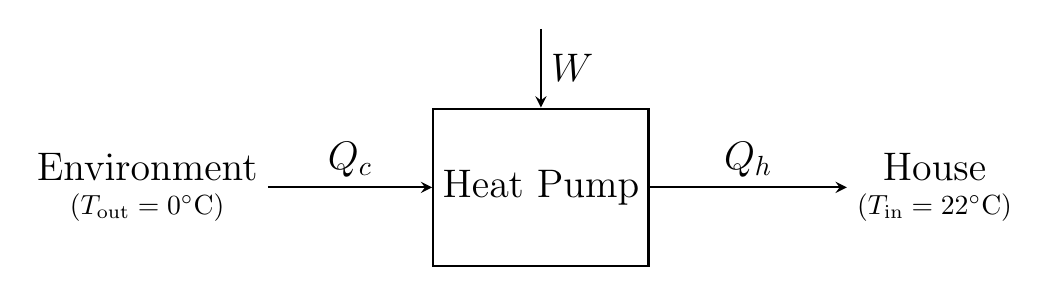
\begin{tikzpicture}[>=stealth,thick]

    % -- Nodes for Environment, Heat Pump, House --
    % Environment on the left
    \node[align=center] (env) at (0,0) 
        {\Large Environment\\($T_{\text{out}} = 0^\circ\mathrm{C}$)};
  
    % Heat pump in the center as a rectangle
    \node[draw, minimum width=2.5cm, minimum height=2cm, 
          align=center] (hp) at (5,0) {\Large Heat Pump};
  
    % House on the right
    \node[align=center] (house) at (10,0) 
        {\Large House\\($T_{\text{in}} = 22^\circ\mathrm{C}$)};
  
    % -- Arrows for heat and work flows --
    % Q_c from Environment to Heat Pump
    \draw[->] (env.east) -- node[midway,above]
        {\Large $Q_c$} (hp.west);
  
    % W (work) from above into the Heat Pump
    \draw[->] ($(hp.north)+(0,1)$) -- 
              node[right] {\Large $W$} (hp.north);
  
    % Q_h from Heat Pump to House
    \draw[->] (hp.east) -- node[midway,above]
        {\Large $Q_h$} (house.west);
  
  \end{tikzpicture}

  \section*{First Law for a Heat Pump}

\subsection*{Conceptual Picture}

A \textit{heat pump} transfers heat from the cold outdoors (temperature $T_C$) into the warmer indoors (temperature $T_H$). To do so, it requires an input of work $\displaystyle W_{\text{on}}$.

\begin{itemize}
    \item $\displaystyle Q_C$: heat extracted from the cold reservoir (outside air).
    \item $\displaystyle W_{\text{on}}$: work input to the heat pump.
    \item $\displaystyle Q_H$: heat delivered to the hot reservoir (the house).
\end{itemize}

In steady-state operation, the internal energy of the working fluid (the refrigerant) does not change. Hence, by the First Law of Thermodynamics:
\[
\Delta U = 0 
\quad \Longrightarrow \quad 
(\text{Energy In}) - (\text{Energy Out}) = 0.
\]

\subsection*{Mathematical Expression}

From the perspective of the heat pump:
\[
\underbrace{Q_H}_{\text{heat to house}} 
= \underbrace{Q_C}_{\text{heat from cold reservoir}}
+ \underbrace{W_{\text{on}}}_{\text{work input}}.
\]

This is the key relationship for a heat pump.  
It tells us that the total heat delivered to the house ($Q_H$) is the sum of the work input ($W_{\text{on}}$) \emph{plus} the heat extracted from the cold outside air ($Q_C$).

\subsection*{Answer}

\[
\boxed{ Q_H = Q_C + W_{\text{on}} }.
\]
\section*{Minimum Work for an Ideal Heat Pump}

\paragraph{Given:}
\begin{itemize}
  \item The house interior is at $T_{\text{hot}} = 22^\circ\mathrm{C} = 295\,\mathrm{K}$.
  \item The outside (cold reservoir) is at $T_{\text{cold}} = 0^\circ\mathrm{C} = 273\,\mathrm{K}$.
  \item The house loses heat at a rate of $15\,\mathrm{kW}$ (i.e.\ $Q_h = 15\,\mathrm{kJ/s}$).
\end{itemize}
We wish to find the \emph{minimum} power $W$ the heat pump must supply to transfer $Q_h=15\,\mathrm{kW}$ from $T_{\text{cold}}$ to $T_{\text{hot}}$.  

\subsection*{Step 1: Coefficient of Performance for an Ideal Heat Pump}
For a reversible (Carnot) heat pump, the coefficient of performance (COP) when delivering heat to the hot reservoir at $T_{\text{hot}}$ is
\[
\mathrm{COP}_{\text{hp}}
\,=\, \frac{Q_h}{W}
\,=\, \frac{T_{\text{hot}}}{T_{\text{hot}} - T_{\text{cold}}},
\]
with absolute temperatures (in Kelvin).

\subsection*{Step 2: Numerical Value of the COP}
Substitute:
\[
T_{\text{hot}} = 295\,\mathrm{K}, 
\quad
T_{\text{cold}} = 273\,\mathrm{K}.
\]
Hence
\[
\mathrm{COP}_{\text{hp}}
= \frac{295}{295 - 273}
= \frac{295}{22}
\approx 13.41.
\]

\subsection*{Step 3: Minimum Power Required}
Because $\mathrm{COP}_{\text{hp}} = Q_h / W$, we solve for the work $W$:
\[
W \;=\; \frac{Q_h}{\mathrm{COP}_{\text{hp}}}.
\]
Given the house requires $Q_h = 15\,\mathrm{kW}$ of heat to stay at $22^\circ\mathrm{C}$,
\[
W 
= \frac{15\,\mathrm{kW}}{13.41}
\;\approx\; 1.12\,\mathrm{kW}.
\]
This is the \emph{minimum} power required for a \emph{reversible} heat pump operating between $273\,\mathrm{K}$ and $295\,\mathrm{K}$ to supply $15\,\mathrm{kW}$ of heat to the house.

\subsection*{Interpretation}
\begin{itemize}
  \item \textbf{In one second}: The pump would consume about $1.12\,\mathrm{kJ}$ of work (since power is kJ/s).
  \item \textbf{On an ongoing basis}: The pump must be rated at $1.12\,\mathrm{kW}$ of power if the house loses $15\,\mathrm{kW}$ of heat continuously.
\end{itemize}
In reality, no heat pump is perfectly reversible, so the actual required power would be higher.

\section*{Answer}
\[
\boxed{W_{\min} \approx 1.12\,\mathrm{kW} \quad (\text{ideal, reversible heat pump}).}
\]

\section*{Heat Pump: Choosing Between Outside Air vs. Ground}

\subsection*{Figure of Merit: \texorpdfstring{$W_{\text{on}}/Q_{\text{leak}}$}{W on / Q leak}}

A convenient way to characterize a heat pump is the ratio
\[
\frac{W_{\text{on}}}{Q_{\text{leak}}},
\]
where 
\begin{itemize}
  \item $W_{\text{on}}$ is the required input \emph{power} (i.e., rate of doing work) to drive the heat pump,
  \item $Q_{\text{leak}}$ is the rate of heat loss from the house that needs to be replaced.
\end{itemize}
\noindent
The smaller this ratio, the more efficient (lower power required for the same heat delivery).

\subsection*{Key Thermodynamic Insight (COP for a Reversible Heat Pump)}

For an ideal (Carnot) heat pump operating between a hot reservoir at $T_H$ (the house temperature) and a cold reservoir at $T_C$ (outside air, ground, etc.), the \textbf{Coefficient of Performance} (COP) is
\[
\text{COP}
= \frac{Q_H}{W_{\text{on}}}
= \frac{T_H}{T_H - T_C},
\]
where $T_H$ and $T_C$ are in \textbf{Kelvin}.

\subsection*{Comparing Heat Sources: Ground vs. Outside Air}

\begin{itemize}
  \item \textbf{House:} $T_H = 22^\circ\mathrm{C} \approx 295\,\mathrm{K}.$
  \item \textbf{Ground:} $T_C \approx 5^\circ\mathrm{C} \approx 278\,\mathrm{K}.$
  \item \textbf{Outside Air in Winter:} $T_C \approx -20^\circ\mathrm{C} \approx 253\,\mathrm{K}.$
\end{itemize}

\vspace{1em}
\noindent
\textbf{Case 1: Ground Source at 5$^\circ$C}
\[
T_H - T_C
= 295\,\mathrm{K} - 278\,\mathrm{K}
= 17\,\mathrm{K}.
\]
So,
\[
\text{COP}_\text{ground}
= \frac{295}{17}
\approx 17.4.
\]

\noindent
\textbf{Case 2: Air Source at -20$^\circ$C}
\[
T_H - T_C
= 295\,\mathrm{K} - 253\,\mathrm{K}
= 42\,\mathrm{K}.
\]
Thus,
\[
\text{COP}_\text{air}
= \frac{295}{42}
\approx 7.0.
\]

\subsection*{Interpretation}
The COP is higher (in the ideal, reversible limit) when the difference $(T_H - T_C)$ is \emph{smaller}. Drawing heat from ground at $\approx 5^\circ\mathrm{C}$ reduces the temperature lift that the heat pump must overcome compared to the very cold outdoor air at $-20^\circ\mathrm{C}$. A higher COP means:
\[
\text{COP} = \frac{Q_H}{W_{\text{on}}}
\quad \Longrightarrow \quad
\frac{W_{\text{on}}}{Q_H} = \frac{1}{\text{COP}}.
\]
Hence, if $\text{COP}_\text{ground} \gg \text{COP}_\text{air}$, the same $Q_H$ (heat needed to replace the house's heat leak) requires:
\[
W_{\text{on}}^\text{(ground)} 
< W_{\text{on}}^\text{(air)}.
\]

\subsection*{Conclusion}
\textbf{It is generally better to use ground-source heat (about 5$^\circ$C) rather than air-source heat (often below -20$^\circ$C in winter) because the smaller temperature difference ($T_H - T_C$) results in a higher COP. This means less input work is needed for the same heating load.}

\end{document}
